\documentclass[10pt,twocolumn,letterpaper]{article}
\usepackage{cvpr}
\usepackage{graphicx,amsmath,amssymb,booktabs,xcolor}
\usepackage[shortlabels]{enumitem}
\usepackage[pagebackref,breaklinks,colorlinks]{hyperref}
\usepackage[capitalize]{cleveref}
\usepackage{tikz}
\usetikzlibrary{arrows.meta,positioning,fit}
\def\cvprPaperID{AIGCIC2026}
\def\confName{ECCV LoViF Workshop}
\def\confYear{2026}

\begin{document}
\title{Rate-Adaptive One-Step Diffusion Compression for AIGC Images\\LoViF 2026 Challenge Factsheet}
\author{Nitiz Khanal\\Pulchowk Campus, Lalitpur, Nepal\\{\tt\small khanalnitij20@gmail.com}}
\maketitle

\begin{abstract}
This factsheet documents our final entry to the LoViF 2026 AIGC Image Compression Challenge. The system combines a learned entropy model with a one-step diffusion reconstruction prior, four rate-specialized codec checkpoints, encoder-side latent refinement, and a fixed lightweight decoder-side restoration network. A per-image rate allocation step chooses among valid entropy-coded candidates while respecting the global 0.025 bits-per-pixel (BPP) constraint. The submitted decoder is source-independent: it reconstructs an image using only its bitstream, the submitted checkpoints, and fixed pretrained components. The final archive corresponds to the team's Codabench final-test entry with organizer-recalculated score 31.527739.
\end{abstract}

\section{Introduction}
The LoViF 2026 AIGC Image Compression Challenge studies ultra-low-bitrate coding under a strict global rate constraint, with distortion, perceptual reconstruction quality, semantic consistency, and compact representations evaluated together. This setting is especially demanding for generated images containing typography, synthetic edges, repeated motifs, UI-like layouts, and stylized texture. At very low rate, conventional codecs tend to erase these structures, while unconstrained generative reconstruction can change their geometry or meaning.

Our contribution is a rate-adaptive learned codec that combines practical entropy coding, a one-step diffusion reconstruction prior, rate-specialized checkpoints, encoder-side latent refinement, exact aggregate rate allocation, and a conservative decoder-side residual restorer. All selected streams are independently decodable by the codec and fixed checkpoints submitted during the Code Submission Phase. The final results, bitstreams, reconstructed images, and this factsheet are supplied for ranking verification and challenge-report use.

\section{Factsheet Information}
\subsection{Team details}
Nitiz Khanal is the sole team member. The email below is the email that should be associated with the corresponding OpenReview profile before submission.
\begin{table}[h]
\centering\footnotesize
\begin{tabular}{@{}ll@{}}
\toprule
Team & ZeroR \\
Team leader & Nitiz Khanal \\
Affiliation & Pulchowk Campus, Lalitpur, Nepal \\
Email & \texttt{khanalnitij20@gmail.com} \\
Alternative email & \texttt{077bel025.nitiz@pcampus.edu.np} \\
Codabench team/user & ZeroR / nitizkhanal \\
OpenReview profile & \texttt{\string~Nitiz\_Khanal1} \\
Team website & Not applicable \\
Source/executable & \textbf{[insert submitted-decoder link]} \\
Results/bitstreams & \textbf{[insert final ZIP link]} \\
Final result archive & \texttt{submission\_test.zip} \\
Official final score & 31.527739 \\
\bottomrule
\end{tabular}
\caption{Team and final-entry identification. Bracketed identity fields must be confirmed before emailing the organizers.}
\end{table}

The entry targets the AIGC track and follows the required result layout: one reconstructed PNG and one independently decodable binary stream for every test image, plus the runtime metadata file. The corresponding decoder and checkpoints were submitted during the Code Submission Phase and were not updated for final-test generation.

\subsection{Method details}
\subsubsection{Design motivation}
At 0.025 BPP, a conventional distortion-oriented codec tends to remove precisely the structures that distinguish generated imagery: typography, synthetic edges, repeated patterns, UI-like regions, and stylized micro-texture. A purely generative decoder can restore plausible texture, but may move edges or change symbols and therefore lose PSNR. Our design treats this as a rate--perception allocation problem. The entropy-coded latent preserves compact structural evidence, while a frozen one-step diffusion prior supplies a strong image manifold. Encoder-side optimization then adapts the latent to each source image without altering any decoder parameters.

\subsubsection{Overall framework and pipeline}
Figure~\ref{fig:pipeline} summarizes the submitted system. Four rate-specialized AEIC-ME checkpoints share the same decoding topology but operate at different rate/perception points. For each image, the encoder evaluates admissible candidates, performs latent test-time optimization (TTO), entropy-codes the refined latent using practical rANS coding, and records a one-byte checkpoint identifier. A global multiple-choice knapsack optimizer selects one candidate per image under the exact aggregate bit budget. At the decoder, the identifier selects the corresponding checkpoint; a tiled one-step diffusion reconstruction is followed by a fixed residual restoration CNN.

\begin{figure*}[t]
\centering
\resizebox{0.98\textwidth}{!}{%
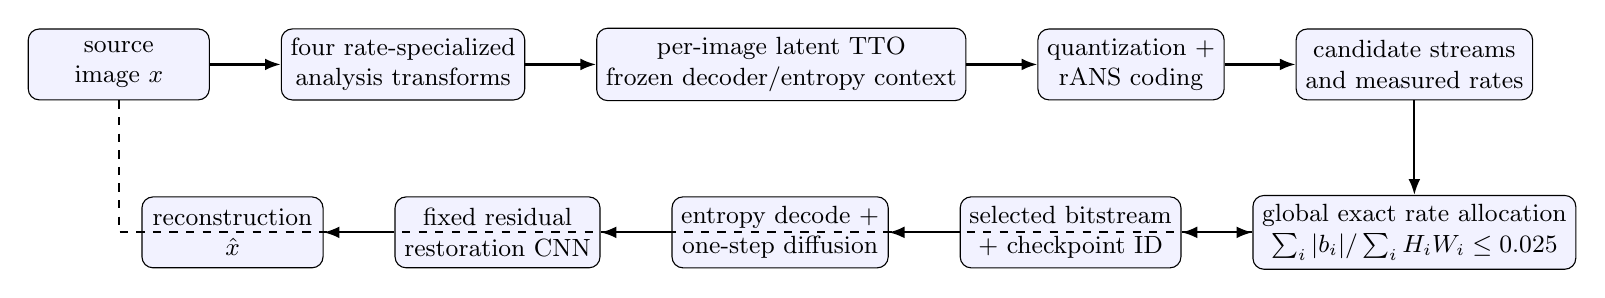
\begin{tikzpicture}[font=\small, node distance=7mm and 9mm,
 box/.style={draw,rounded corners,align=center,minimum height=9mm,minimum width=23mm,fill=blue!5},
 arr/.style={-{Latex[length=2mm]},thick}]
\node[box] (src) {source\\image $x$};
\node[box,right=of src] (multi) {four rate-specialized\\analysis transforms};
\node[box,right=of multi] (tto) {per-image latent TTO\\frozen decoder/entropy context};
\node[box,right=of tto] (rans) {quantization +\\rANS coding};
\node[box,right=of rans] (pool) {candidate streams\\and measured rates};
\node[box,below=12mm of pool] (knap) {global exact rate allocation\\$\sum_i |b_i|/\sum_i H_iW_i\leq0.025$};
\node[box,left=of knap] (stream) {selected bitstream\\+ checkpoint ID};
\node[box,left=of stream] (dec) {entropy decode +\\one-step diffusion};
\node[box,left=of dec] (enh) {fixed residual\\restoration CNN};
\node[box,left=of enh] (out) {reconstruction\\$\hat{x}$};
\draw[arr] (src)--(multi); \draw[arr] (multi)--(tto); \draw[arr] (tto)--(rans);
\draw[arr] (rans)--(pool); \draw[arr] (pool)--(knap); \draw[arr] (knap)--(stream);
\draw[arr] (stream)--(dec); \draw[arr] (dec)--(enh); \draw[arr] (enh)--(out);
\draw[arr,dashed] (src.south) |- (knap.west);
\end{tikzpicture}}
\caption{Final compression pipeline. Dashed flow denotes encoder-only access to the source for candidate evaluation and rate allocation. The submitted decoder receives only the selected bitstream.}
\label{fig:pipeline}
\end{figure*}

\subsubsection{Network architecture and advanced prior}
The base is the ME variant of the AEIC learned image codec. Its analysis side maps RGB content into a compact quantized latent governed by a learned autoregressive entropy model. The synthesis path conditions an SD-Turbo one-step diffusion network~\cite{sauer2023sdturbo} on the decoded latent. SD-Turbo provides a high-capacity perceptual prior while avoiding the runtime of iterative diffusion sampling. The decoder uses the submitted trimmed FP16 SD-Turbo UNet and VAE components together with the AdcSR half-decoder used by the AEIC implementation. CompressAI~\cite{begaint2020compressai} supplies supporting learned-compression primitives.

Four fine-tuned checkpoints cover complementary operating regions. Their binary streams share one decoder entry point; the first byte selects the checkpoint, after which the remaining payload is decoded by the practical entropy coder. This explicit signaling makes per-image model selection reproducible and adds negligible overhead. Large images are reconstructed using overlapping latent and VAE tiles. Overlap is larger than the effective local receptive boundary, reducing seams while keeping peak activation memory bounded.

The final restoration module is an eight-block residual CNN with dense local feature reuse. It predicts a bounded RGB residual and is identity-initialized through a zero-initialized final convolution. It does not consume source pixels or side information and adds zero BPP. Its purpose is conservative correction of recurring color, edge, and local texture errors rather than unconstrained detail generation.

\subsubsection{Bitstream generation, entropy coding, and rate control}
All reported rates use real coded files rather than entropy estimates. Let candidate $j$ for image $i$ have score $s_{ij}$ and stream length $r_{ij}$ bits. Final selection solves
\begin{align}
 \max_{z_{ij}}\;&\sum_{i,j}s_{ij}z_{ij},\\
 \text{s.t. }&\sum_jz_{ij}=1,\quad
 \sum_{i,j}r_{ij}z_{ij}\leq0.025\sum_iH_iW_i.
\end{align}
with binary $z_{ij}$. The optimization uses the exact file sizes, including model identifiers and stream headers. This is important because low-rate images can have non-negligible fixed overhead and because images have different spatial dimensions.

\subsubsection{Perceptual reconstruction and encoder-side refinement}
For each candidate checkpoint, TTO refines the continuous latent while freezing the decoder weights and entropy-model conditioning. We use Adam for 300 steps. The objective combines pixel distortion and perceptual terms,
\begin{equation}
 \mathcal{L}_{\mathrm{TTO}}=\lambda_2\|x-\hat{x}\|_2^2+\lambda_L\mathcal{L}_{\mathrm{LPIPS}}+\lambda_D\mathcal{L}_{\mathrm{DISTS}}+\lambda_R R.
\end{equation}
The final quantized latent is passed through the actual entropy encoder. Freezing autoregressive conditioning during a refinement trajectory improves stability, while final re-encoding ensures that the submitted payload remains a genuine decodable stream. TTO is strictly an encoder operation; the final decoder performs no optimization or online fine-tuning.

\subsubsection{Training data}
We used the 800 challenge-provided AIGC training images. We additionally generated approximately 15.7k synthetic AIGC images from public prompt collections representing GenEval, DPG-Bench, CVTG-2K, and LongText-Bench styles. Generation used publicly available SDXL, SD3.5-medium, PixArt-Sigma, and Sana models. The external corpus was used only for codec/domain fine-tuning and restoration training. Challenge validation and test images were not used for gradient updates, checkpoint fitting, or decoder adaptation. Thus, \textbf{extra training data was used and is disclosed here}.

Training samples were randomly cropped and horizontally flipped. Mixed image sources and multiple codec-rate reconstructions were sampled so that the restoration module did not specialize to a single rate point. The training pipeline rejected invalid/corrupt images and retained RGB images large enough for the configured crop.

\subsubsection{Training strategy and optimization protocol}
Codec fine-tuning started from the public AEIC-ME checkpoint and retained the public SD-Turbo/AdcSR initialization. Rate-specialized models were produced by varying rate and reconstruction weights, rather than training unrelated architectures. Training used Adam/AdamW-family optimization with cosine learning-rate decay; the initial learning rate was approximately $2\times10^{-4}$ for the small restoration module. Restoration batches used random patches (up to $384\times384$ depending on the experiment) and batch size 8. Gradients were clipped to unit norm.

The restoration loss combined L1/pixel error, LPIPS, DISTS, and an edge-aware DISTS term. Adversarial loss was evaluated during development but was disabled in the final conservative model because it could improve apparent sharpness while damaging distortion and text fidelity. Checkpoints were evaluated using actual reconstructed validation images and real stream lengths. Model selection considered PSNR, MS-SSIM, LPIPS, DISTS, BPP, and decoder reproducibility jointly.

\subsubsection{Experimental results}
The challenge combines distortion, structural similarity~\cite{wang2003msssim}, LPIPS~\cite{zhang2018lpips}, and DISTS~\cite{ding2020dists}. The official test-phase page specifies
\begin{equation}
S=\mathrm{PSNR}+10\,\mathrm{MS\mbox{-}SSIM}+40(1-\mathrm{LPIPS})+40(1-\mathrm{DISTS}),
\end{equation}
where lower LPIPS and DISTS are better and higher PSNR and MS-SSIM are better. Table~\ref{tab:results} records the score displayed for the final Codabench entry; the organizer's archived evaluation and ranking procedure remain authoritative.

\begin{table}[h]
\centering\small
\begin{tabular}{@{}lc@{}}
\toprule
Quantity & Final test entry \\
\midrule
Final score & 31.527739 \\
PSNR & 27.022356 dB \\
MS-SSIM & 0.917594 \\
LPIPS & 0.077794 \\
DISTS & 0.038970 \\
Average BPP & 0.024946 \\
Reported runtime & 8.5 s/image \\
Execution device & GPU \\
\bottomrule
\end{tabular}
\caption{Official organizer-recalculated final-test metrics announced on August 4, 2026.}
\label{tab:results}
\end{table}

The result is strongest on perceptual structure, particularly DISTS, while PSNR remains the principal limitation. This behavior is expected for a diffusion-assisted reconstruction method at ultra-low rate. The multi-model allocation prevents a single rate point from dominating images for which it is poorly matched and was consistently more effective than selecting one checkpoint globally.

\subsubsection{Complexity, runtime, and reproducibility}
Encoding uses one NVIDIA GPU and is dominated by 300-step per-image latent refinement. The submitted metadata reports 8.5 seconds per image in the evaluation environment used for the final archive. Decoding performs one entropy decode, one one-step diffusion reconstruction, and one restoration-CNN pass; no test-time gradient computation is required. Tiled execution bounds memory on large inputs. The submitted decoder bundle contains the trimmed FP16 SD-Turbo UNet/VAE, AdcSR half-decoder, four AEIC-ME checkpoints, restoration weights, practical entropy-coding extension, inference scripts, dependency notes, and a README.

Reproduction requires Python 3.10, PyTorch 2.1.x with CUDA 12.x-compatible runtime, CompressAI 1.2.8, Diffusers, xFormers, and the compiled rANS extension included by the build procedure. For each stream, the standalone decoder reads its checkpoint byte, loads the corresponding codec, entropy-decodes the latent, performs tiled synthesis, applies the fixed restorer, clamps to $[0,1]$, and writes an RGB PNG. No original image, prompt, internet service, or hidden metadata is required.

The final test-results ZIP has been CRC-validated and contains 100 reconstructed images, 100 binary streams, and one metadata/readme file. Its total size is 298,889,715 bytes (approximately 299 MB, or 285 MiB). The binary streams themselves occupy 742,548 bytes in total: 7,425.48 bytes/image on average, with a minimum of 2,092 and maximum of 16,525 bytes. Their pixel-weighted rate is 0.0250 BPP.

Separately, the decoder and checkpoint bundle supplied during the earlier Code Submission Phase is approximately 4.76 GB unpacked, under the 5 GB decoder limit. This is not the final test-results ZIP described above. The decoder bundle's principal components are approximately 2.46 GB of four codec checkpoints, 1.90 GB of trimmed FP16 SD-Turbo weights, 0.38 GB of AdcSR weights, and a small restoration model plus code. Peak GPU allocation observed for large tiled reconstructions was approximately 11.4 GB. A formal architecture-independent FLOP count was not measured because entropy decoding, attention, and content-dependent tiling make a single FLOP figure misleading; runtime and memory are reported directly instead. Typical decode time was approximately 1--2 seconds for ordinary images and higher for the largest tiled inputs. The submitted challenge metadata reports the complete per-image pipeline runtime as 8.5 seconds on GPU.

\subsubsection{Pretrained models, comparisons, and originality}
External pretrained components are SD-Turbo, the AdcSR half-decoder, and the public AEIC-ME initialization; all required inference weights are included in the submitted decoder bundle. Our main originality is the practical integration of a one-step generative prior with exact real-stream rate allocation and stable per-image latent refinement for AIGC content. Unlike an output ensemble, the method sends exactly one valid bitstream per image. Development comparisons found that generic distortion-oriented codecs could improve PSNR on some images but caused much worse LPIPS and DISTS, whereas the submitted method retained stronger perceptual structure.

\section{Ensembles and Multi-Model Strategies}
The method is a multi-model rate ensemble, not an output-image ensemble. Exactly one candidate stream and one checkpoint are selected for each image. No pixel averaging, oracle information, or multiple decoder outputs are used at evaluation time. All four checkpoint choices and the selection signaling were part of the codec submitted for reproducibility. The global allocator is encoder-only and uses source-reference metrics solely to choose among streams that the submitted decoder can independently reconstruct.

\subsection{Component roles and ablations}
Development experiments showed three recurring effects. First, deeper latent refinement improved the aggregate rate--perception objective but eventually showed diminishing returns. Second, the fixed residual restorer yielded a small but reliable zero-rate gain when trained on reconstructions matching the final codec distribution. Third, generic distortion-oriented codecs could improve PSNR on selected content but produced substantially worse LPIPS/DISTS on this AIGC test distribution; consequently, they were not used in the submitted final codec. We also found that source-dependent fallback logic must be explicitly excluded: every selected reconstruction was checked for bitstream-only decoder reproducibility.

\section{Other details}
\subsection{Workshop plans and challenge feedback}
The challenge usefully exposes a real tension between distortion and perceptual preservation in generated imagery. Future editions could report separate objective and perceptual rankings directly, publish the exact aggregation/tie-breaking rules, and provide a standardized decoder container with deterministic CUDA/tiled-inference tolerances. A small text-legibility or OCR-sensitive metric would also complement PSNR, MS-SSIM, LPIPS, and DISTS for poster-like AIGC content.

\section*{Compliance Statement}
This document describes the codec and pretrained checkpoints submitted for the Code Submission Phase. The final test archive was generated using that corresponding submitted codec. No decoder model update, retraining, or online/test-time model fine-tuning was performed after the Code Submission Phase. Encoder-side latent optimization is part of the submitted compression procedure and does not modify decoder weights.

{\small
\bibliographystyle{ieeenat_fullname}
\bibliography{egbib}
}
\end{document}
